\documentclass[11pt]{article}
\usepackage{common}
\usepackage[usenames, dvipsnames]{color}
\usepackage{setspace}
\usepackage{booktabs}
\usepackage{multirow}
\usepackage{framed}

\title{CS207 Algorithm Analysis: Kernel Density Estimation}
\author{Gioia Domined\`o \and Nicolas Drizard \and Kendrick Lo}

\begin{document}
\maketitle{}

\pagestyle{plain}
\pagenumbering{arabic}

\section{Introduction}

Kernel Density Estimation (KDE) is a non-parametrical statistical technique that is used to estimate the probability density function (PDF) of a random variable based on a finite data sample\footnote{https://en.wikipedia.org/wiki/Kernel\_density\_estimation}.  Mathematically, we can denote the estimated PDF of independent and identically distributed (\textit{iid}) random variables $X=\{x_1, x_2, ..., x_n\}$ as:

\begin{equation} \label{eq:kde}
\hat{f}_h(x) = \frac{1}{n} \sum_{i=1}^n K_h(x - x_i) = \frac{1}{nh} \sum_{i=1}^n K \Big( \frac{x - x_i}{h} \Big)
\end{equation}

\noindent where $K(\cdot)$ represents the \textit{kernel} and $h$ represents the \textit{bandwidth} (i.e. a smoothing parameter). We note that $\hat{f}_h(x)$ denotes the estimated PDF at a particular point $x$, and that the entire data set $X$ is used to calculate it. \medskip

\noindent Various kernels are used in practice (e.g. Gaussian, Epanechnikov, exponential, etc.), all of which meet the criteria of being non-negative functions with mean zero that integrate to one. Similarly, different (strictly positive) values of $h$ can be chosen depending on the data set in question. Figure \ref{fig:kde_params} illustrates how the choice of these two parameters affects the shape of the estimated PDF.

\begin{figure}[h!]
\centering
\subfloat[Changing the kernel (bandwidth$=0.2$)]{\label{fig:kde_params_k}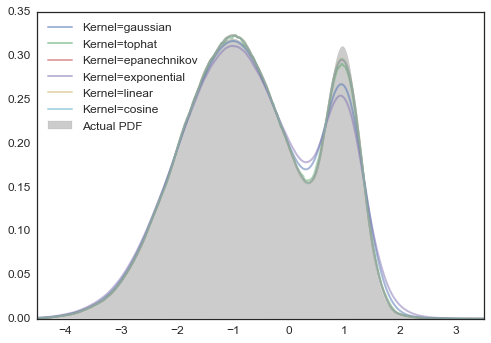
\includegraphics[width=3in]{img/change_k}}
\subfloat[Changing the bandwidth (gaussian kernel)]{\label{fig:kde_params_bw}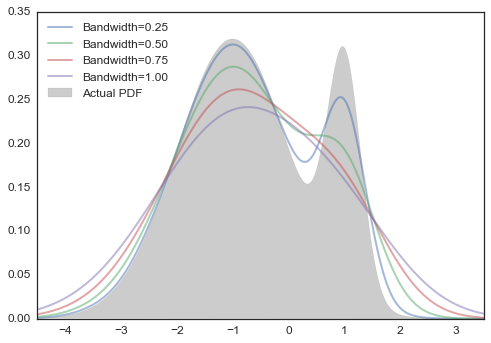
\includegraphics[width=3in]{img/change_bw}}
\caption{Impact of KDE parameters}
\label{fig:kde_params}
\end{figure}

\newpage

\section{Pure Python Algorithm}

A discussion on the ``best" parameters\footnote{In addition to the parameters discussed above, different distance metrics may also be employed.} for KDE is beyond the scope of this paper.  For ease of comparability, all our experiments are based on a Gaussian kernel and a bandwidth of $0.2$. Figure \ref{fig:sample_kde} shows the result of running the Scikit-Learn KDE algorithm with these parameters on 100K one-dimensional random variables drawn from a bimodal distribution, where the PDF is plotted at 1K evenly-spaced values of $x$.

\begin{figure}[h!]
\centering
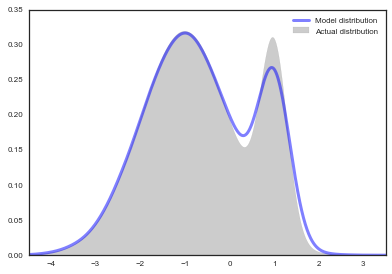
\includegraphics[width=3in]{img/sample_kde.png}
\caption{Sample KDE output}
\label{fig:sample_kde}
\end{figure}

\paragraph{Na\"ive Python KDE.} We started by implementing a "pure" Python version of KDE that only uses lists\footnote{All code is available at https://github.com/Mynti207/algo-paper/blob/master/code/KDE\_python.ipynb.}.  The implementation \textendash \ which is a direct application of Equation \ref{eq:kde} \textendash \ is presented in the code blocks below. The double loop is necessary due to the use of lists, and immediately stands out as a significant source of inefficiencies.

\begin{framed}
\begin{singlespacing}
\begin{scriptsize}
\begin{verbatim}
def gaussian(x):
    '''
    Returns the Gaussian function for a given input variable.
    
    Parameters
    ----------
    x : Float, the x-value at which to evaluate the Gaussian function
        
    Returns
    ----------
    The result of evaluating the Gaussian function at x
    '''
    return np.exp(-1.0 * (x**2) / 2) * (1.0 / np.sqrt(2.0 * np.pi))
\end{verbatim}
\end{scriptsize}
\end{singlespacing}
\end{framed}

\newpage

\begin{framed}
\begin{singlespacing}
\begin{scriptsize}
\begin{verbatim}
def naive_kde(x, x_grid, h):
    '''
    Calcalates the KDE PDF estimate, based on a Gaussian kernel.
    
    Parameters
    ----------
    x : A list of iid random variables that are used to calculate the KDE estimate
    x_grid : A list of values along which to calculate the KDE estimate
    h : Float, the bandwidth parameter for the KDE estimate
        
    Returns
    ----------
    A list of KDE estimates for all values of x_grid
    '''
    global N # number of iid random variables
    estimates = [0] * len(x_grid)
    
    for j, gridpt in enumerate(x_grid):
        for i in range(N):
            val_in_sum = gaussian((x[i] - gridpt) / h)
            estimates[j] += val_in_sum
        
        estimates[j] = estimates[j] / (N * h)
    
    return estimates
\end{verbatim}
\end{scriptsize}
\end{singlespacing}
\end{framed}

\paragraph{Vectorized Python KDE.} Before moving on to Scikit-Learn, we tested the effect of switching from lists to Numpy arrays and vectorizing the inner loop. This simple change, which is shown in the code below, reduced the runtime from over 300 seconds to just over 1 second!

\begin{framed}
\begin{singlespacing}
\begin{scriptsize}
\begin{verbatim}
def vectorized_kde(x, x_grid, h):
    '''
    Calcalates the KDE PDF estimate, based on a Gaussian kernel.
    Inputs
    ----------
    x      : An array of iid random variables that are used to calculate the KDE estimate
    x_grid : An array of values along which to calculate the KDE estimate
    h      : Float, the bandwidth parameter for the KDE estimate
    Returns
    ----------
    An array of KDE estimates for all values of x_grid
    '''    
    global N # number of iid random variables

    estimates = np.zeros(len(x_grid))
    
    for j, gridpt in enumerate(x_grid):
        val_in_sum = gaussian((x - gridpt)/h)  # returns vector of dim N
        estimates[j] = np.sum(val_in_sum) / (N * h)
    
    return estimates
\end{verbatim}
\end{scriptsize}
\end{singlespacing}
\end{framed}

\newpage

\section{Scikit-Learn Algorithm}

After completing our Python implementations, we next moved on to examine the Scikit-Learn implementation\footnote{The full source code is available at https://github.com/scikit-learn/scikit-learn/tree/master/sklearn/neighbors.} and analyze its optimizations. It is not surprising that the developers of alternative implementations would want to improve upon the efficiency of a pure Python approach; in particular, it is clear that an algorithm of low(er) complexity is particularly desirable as the problem scales by increasing the size of the input dataset and/or the number of points along which the PDF is being estimated. \medskip

\noindent The Scikit-Learn KDE implementation incorporates two main optimizations: \textit{Cython implementations} and \textit{tree-based computational methods}.

\paragraph{Cython.} Cython is an extension-module generator for Python that allows code to be written in Python \textendash \ with the added requirement that type declarations be made explicit \textendash \ and then pre-compiled into an extension module. In this manner, Cython translates the modified Python code into a format that compiles into reasonably fast C code. \medskip

\noindent C is a popular programming language; due to the fact that it is compiled, it is generally (much) faster than Python. In fact, many Numpy operations are implemented in C, thus avoiding ``the general cost of loops in Python, pointer indirection and per-element dynamic type checking"\footnote{See, for example, http://stackoverflow.com/questions/8385602/why-are-numpy-arrays-so-fast.}. The speed of C code is illustrated by the significantly improved runtime of our vectorized Python implementation, which is Numpy-based, compared to our na\"ive Python implementation. Numpy provides significant improvements in execution time for basic KDE calculations; however, it is important to note that not all operations can be vectorized and that the extent of performance improvements may therefore vary. \medskip

\noindent Despite the enhanced performance that generally results from C implementations, C code is lower-level. Consequently, C programming is typically slower and more cumbersome than Python programming. The use of Cython can therefore be seen as a reasonable compromise between performance and ease of coding. \medskip

\noindent The primary Python module for the Scikit-Learn KDE implementation is \texttt{kde.py}, which imports modules from \texttt{ball\_tree.pyx}\footnote{https://github.com/scikit-learn/scikit-learn/blob/master/sklearn/neighbors/ball\_tree.pyx} and \texttt{kd\_tree.pyx}\footnote{https://github.com/scikit-learn/scikit-learn/blob/master/sklearn/neighbors/kd\_tree.pyx}, both of which are written in Cython. Furthermore, the functions in \texttt{dist\_metrics.pyx} that correspond to different distance computations are also coded in Cython\footnote{https://github.com/scikit-learn/scikit-learn/blob/master/sklearn/neighbors/dist\_metrics.pyx}. \medskip

\noindent In addition to simply being written in Cython, we observed that some of these modules have also been modified to support multi-threading, which further accelerates performance. This is visible in the incorporation of the \texttt{nogil} argument in certain functions.

\newpage

\paragraph{Tree-based computation.} Alternative Python-based KDE implementations are available in the Scipy and Statsmodel packages; however, according to Jake VanderPlas, a key contributor to  Scikit-Learn, none of these alternatives employ tree-based computation\footnote{https://jakevdp.github.io/blog/2013/12/01/kernel-density-estimation/}. We saw above that the na\"ive KDE algorithm requires all pairwise distance computations to be performed; consequently, to quote VanderPlas, KDE can be placed into ``the same category as Nearest Neighbors, N-point correlation functions, and Gaussian Process Regression, all of which are examples of \textit{Generalized N-body problems} which can be efficiently computed using specialized data structures such as a KD Tree"\footnote{Ibid.}. \medskip

\noindent Tree-based methods have the advantage of scaling as $O(n \log n)$, making them more efficient than the $O(n^2)$ ``brute-force" KDE approach (where a distance computation must be made between each input and output pair) as $n$ becomes large. We cannot improve upon VanderPlas' excellent explanation of how tree-based methods enhance performance: \medskip

\begin{quote}
The main idea is this: if you can show that a query point $Q_0$ is geometrically far from a set of training points $\{T_i\}$, then you no longer need to compute every kernel weight between $Q_0$ and the points in $\{T_i\}$: it is sufficient to compute one kernel weight at the average distance, and use that as a proxy for the others. With careful consideration of the bounds on the distances and the maximum error tolerance for the final result, it is possible to greatly reduce the number of required operations for a KDE computation.\footnote{Ibid.}
\end{quote}
 
 \noindent In order words, structures such as a \textit{KD tree} (a binary tree in which every node represents a $k$-dimensional point\footnote{https://en.wikipedia.org/wiki/K-d\_tree}) or a \textit{ball tree} (a binary tree in which every node represents a $D$-dimensional hypersphere that contains a subset of the points to be searched\footnote{https://en.wikipedia.org/wiki/Ball\_tree}) effectively provide a means for \textit{approximating} the exact KDE solution. Accordingly, though performance is enhanced, there exists a trade-off between computational performance and accuracy. The Scikit-Learn implementation allows users to specify their preferred tolerance (the default value is $0$), where larger tolerance generally leads to faster execution. VanderPlas asserts that even a marginal reduction in accuracy \textendash \ for example, allowing errors of $1$ part in $10^8$ \textendash \ can lead to impressive gains in computational efficiency.
 
\section{Comparing Algorithms}

Following our analysis of the na\"ive Python, vectorized Python and Scikit-Learn Python implementations, we concluded by comparing their performance on datasets of different sizes. Figure \ref{fig:compare_kde} shows the relative runtimes of the three implementations on input data sets of $1e^1$, $1e^2$, $1e^3$, $1e^4$, and $1e^5$ random variables. In all cases, the PDF was estimated for 1K evenly-spaced values of $x$. \medskip

\noindent Unsurprisingly, we can see that the na\"ive Python implementation is consistently much slower \textendash \ so much so, that its results had to be presented in a separate graph due to the very different axis scale. As discussed above, the significantly faster runtime of the vectorized Python implementation is a direct result of harnessing the faster C operations provided by the Numpy library.

\newpage

\begin{figure}[h!]
\centering
\subfloat{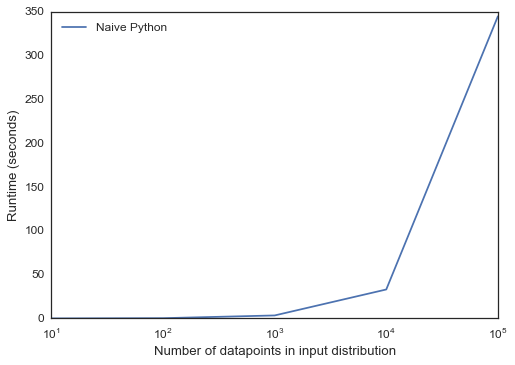
\includegraphics[width=3in]{img/compare_1}}
\subfloat{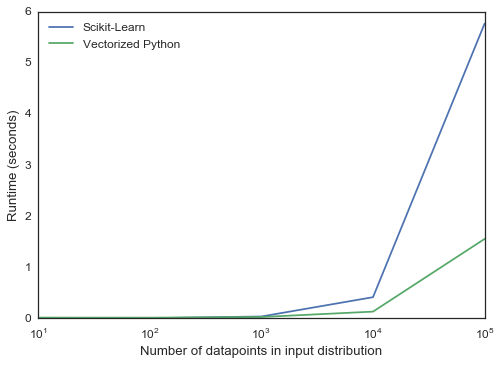
\includegraphics[width=3in]{img/compare_2}}
\caption{Comparing one-dimensional KDE implementations}
\label{fig:compare_kde}
\end{figure}

\noindent Despite its optimizations, the Scikit-Learn algorithm displays slightly longer runtimes that the vectorized Python algorithm. It is important to note that these two implementation are not directly comparable, since the data structures employed and the operations performed are not the same. For example, our vectorized Python implementation avoids the overhead associated with: checking inputs to handle different kernels; and setting up the tree structure. In addition, the vectorized implementation has an advantage in our one-dimensional example, but would not scale as well to larger-dimensional problems. \medskip

\noindent Ultimately, the clearest comparison between implementations is in terms of computational complexity: a ``brute-force" KDE implementation that requires a distance computation to be made between each input and output pair will scale quadratically with $O(n^2)$, while a tree-based implementation will scale logarithmically with $O(n \log n)$.

\end{document}
